\scanpage{80}
\mspage{79}%
valent to $\handwritten{\underline}{G}(\handwritten{\ell})$ for every algebraically closed field $\handwritten{\ell}$ of cha\rlap{\raisebox{-.65em}{r}}racteristic $p\handwritten{>0}$ (to be precise, if $\handwritten{\overline}{\handwritten{\underline}{F}}_p$ is\deleted{\unsure{l|t}} the algebraic closure of $\handwritten{\underline}{F}_p$ in $\handwritten{\ell}$, the inclusion of the latter in $\handwritten{\ell}$ ind\rlap{i}uces an equivalence of \unsure{g|\rlap{e}g}erbes
\[
\handwritten{\underline}{G}(\handwritten{\ell})\handwritten{\underline{\approx}}\handwritten{\underline}{G}(\handwritten{\overline}{\handwritten{\underline}{F}}_p)\deleted{\handwritten{\unsure{)|,}}}\handwritten{\underline{\approx}}\handwritten{\underline}{H}\deleted{\handwritten{\unsure{)|.}}}\qquad ).
\]
8.6. Study of $\operatorname{Rep}(\handwritten{\underline}{H})$. We have said that the classes of simple objects are in one-to-one correspondence with the elements of $\handwritten{\underline}{Q}$ ; the element of $\handwritten{\underline}{Q}$ corresponding to an isotypic object is calle\unsure{\rlap{e}d|d} the \handwritten{\uline}{slope} of this element. We have seen that the object of $\operatorname{Rep}(\handwritten{\underline}{H})$ defined \margin{\handwritten{Notation $E_{s/r}$ for $E_{r,s}$ indicated, hence
\[
E_\lambda\otimes E_{\lambda'}\simeq E_{\lambda\lambda'}^{n(\lambda,\lambda')}
\]
for $\lambda,\lambda'\in\mathbb{Q}$}}
by the object $\handwritten{\underline}{Q}_p[T]/(T^r-p^s)$ of $\operatorname{Fcriso}(\handwritten{\underline}{F}_p)$, equipped with multiplication by $T$, is simple of slope $s/r$ ($s,r\handwritten{\in}\handwritten{\underline}{Z}$, $r\geq1$, $(s,r)=1$ ), so that we thus obtain a complete catalogue of the simple objects $E_{r,s}$. Of course, $E_{r,s}$ is of rank $r$, on the other hand its endomorphism field is \deleted{\unsure{lta|ila}} a skew field \inserted{$K_{r,s}$}\handwritten{\begin{tikzpicture}[baseline=0cm,x=1cm,y=1cm]\draw[thin] (0,0) .. controls (.35,.16) and (.7,.1) .. (1.05,.08) .. controls (1.45,.05) and (1.6,.22) .. (1.64,.48);\end{tikzpicture}} whose class in $\operatorname{Br}(\handwritten{\underline}{Q}_p)=\handwritten{\underline}{Q}/\handwritten{\underline}{Z}$ is $s/r\bmod1$, according to what we saw in 8.3.

$\operatorname{Rep}(\handwritten{\underline}{H})$ is the inductive limit of the full subc\unsure{\rlap{q}a|a}tegories $\operatorname{Rep}(\handwritten{\underline}{H},r)$, $r\geq1$, where $(\handwritten{\underline}{H},r)$ is the quotient of the gerbe $\handwritten{\underline}{H}$ corresponds to the quotient $(H,r)$\handwritten{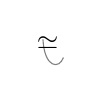
\begin{tikzpicture}[baseline=-.1cm,x=1cm,y=1cm]\draw[gray,thin] (.22,.15)..controls (.24,-.22) and (.43,-.23)..(.48,-.08);\node at (.28,.1) {$\simeq$};\end{tikzpicture}}$\handwritten{\underline}{G}_m$ of its band, such that the Tate homomorphism \deleted{is a} induces a homomorphism $(H,r)\handwritten{\xrightarrow{\unsure{q|a|\alpha}}}\handwritten{\underline}{G}_m$ identified with $x\handwritten{\longmapsto}x^r$ : F-iso\inserted{crystals (over $\handwritten{\overline}{k}$) of slope a multiple of $1/r$.}\handwritten{\begin{tikzpicture}[baseline=0cm,x=1cm,y=1cm]\draw[thin] (0,-.17)..controls (.16,.05) and (.35,.02)..(.62,.02)..controls (.85,.03) and (.95,.08)..(1.05,.12);\end{tikzpicture}} Thus $(\handwritten{\underline}{H},r)$ \deleted{is identified} \unsure{\rlap{a}i|i}\unsure{\rlap{l}s|s}\deleted{\unsure{with|with}} \inserted{a}\handwritten{\begin{tikzpicture}[baseline=0cm,x=1cm,y=1cm]\draw[thin] (0,-.13)--(.65,.13);\end{tikzpicture}} gerbe with band $\handwritten{\underline}{G}_m$, having as its class in $\operatorname{Br}(\handwritten{\underline}{Q}_p)$ th\unsure{\rlap{i}e|e} canonical generator $1/r\bmod\handwritten{\underline}{Z}$ of ${}_r\operatorname{Br}(\handwritten{\underline}{Q}_p)\handwritten{\simeq}\handwritten{\underline}{Z}/r\handwritten{\underline}{Z}$. I\rlap{,}t is also, more canonically, ``the'' gerbe defined by the skew field $K_{r,\handwritten{1}\deleted{s}}$ above, \deleted{which}

\handwritten{[}Amusing exercise, which I have not done: the additive structure of $\operatorname{Rep}(\handwritten{\underline}{H})$ being entirely described by the collection of th\unsure{e|\rlap{z}e} $K_{r,s}$, make its $\handwritten{\otimes}$-structure explicit ... i.e. write the \handwritten{``}canonical relations\handwritten{''} in terms of tensor prod\unsure{\rlap{n}u|u|n}c\unsure{\rlap{e}t|t|e}s between the $E_{r,s}$. Another suggested exercise: find ``canonically'' a description of the Dieudonné modules of the reductions of the Lubin-Tate groups in terms of the $E_{r,s}$ \deleted{\handwritten{\unsure{;|,|.}}} \handwritten{(}in particular, the Lubin-Tate associated with unramified extensions
